\documentclass{beamer}
\usepackage[italian]{babel}
\usepackage[utf8]{inputenc}
\usepackage{default}
\usepackage{subcaption}
\usepackage{afterpage}
\usepackage{xcolor}
\usepackage{wrapfig}
\usepackage{caption}
\usepackage{bbm}
\usepackage{multimedia}

\newsavebox{\tempbox}
\usetheme{Padova}
\title{Local Path Planning with Moving Obstacle Avoidance based on Adaptive MPC in ATLASCAR2}
\subtitle{\itshape Tesi di Laurea in Ingegneria dell'Automazione}
\author{Relatore: Prof. Angelo Cenedese\qquad\quad Laureando: Alberto Franco Correlatore: Prof. Vitor Santos}
\date{\vspace{0.4cm}15 Aprile 2019}

\AtBeginSection[]{
	
	\begin{frame}{}
		\nonumber
		\pagecolor{rossoPantano}\afterpage{\nopagecolor}
		\usebeamerfont{title}\vfill\centering
		\usebeamercolor[fg]{title}\insertsectionhead\par%
		\vfill
	\end{frame}
}

\begin{document}

	\maketitle

	\begin{frame}{Progetto ATLASCAR2}
	  
	  \begin{figure}[!t]
	  	\centering
	  	\begin{minipage}[t]{0.49\textwidth}
		  	
\includegraphics[scale=0.32]{./images/logo_ua.png}
	  		\label{fig:logoua}
	  	\end{minipage}
	  	\begin{minipage}[t]{0.49\textwidth}
	  		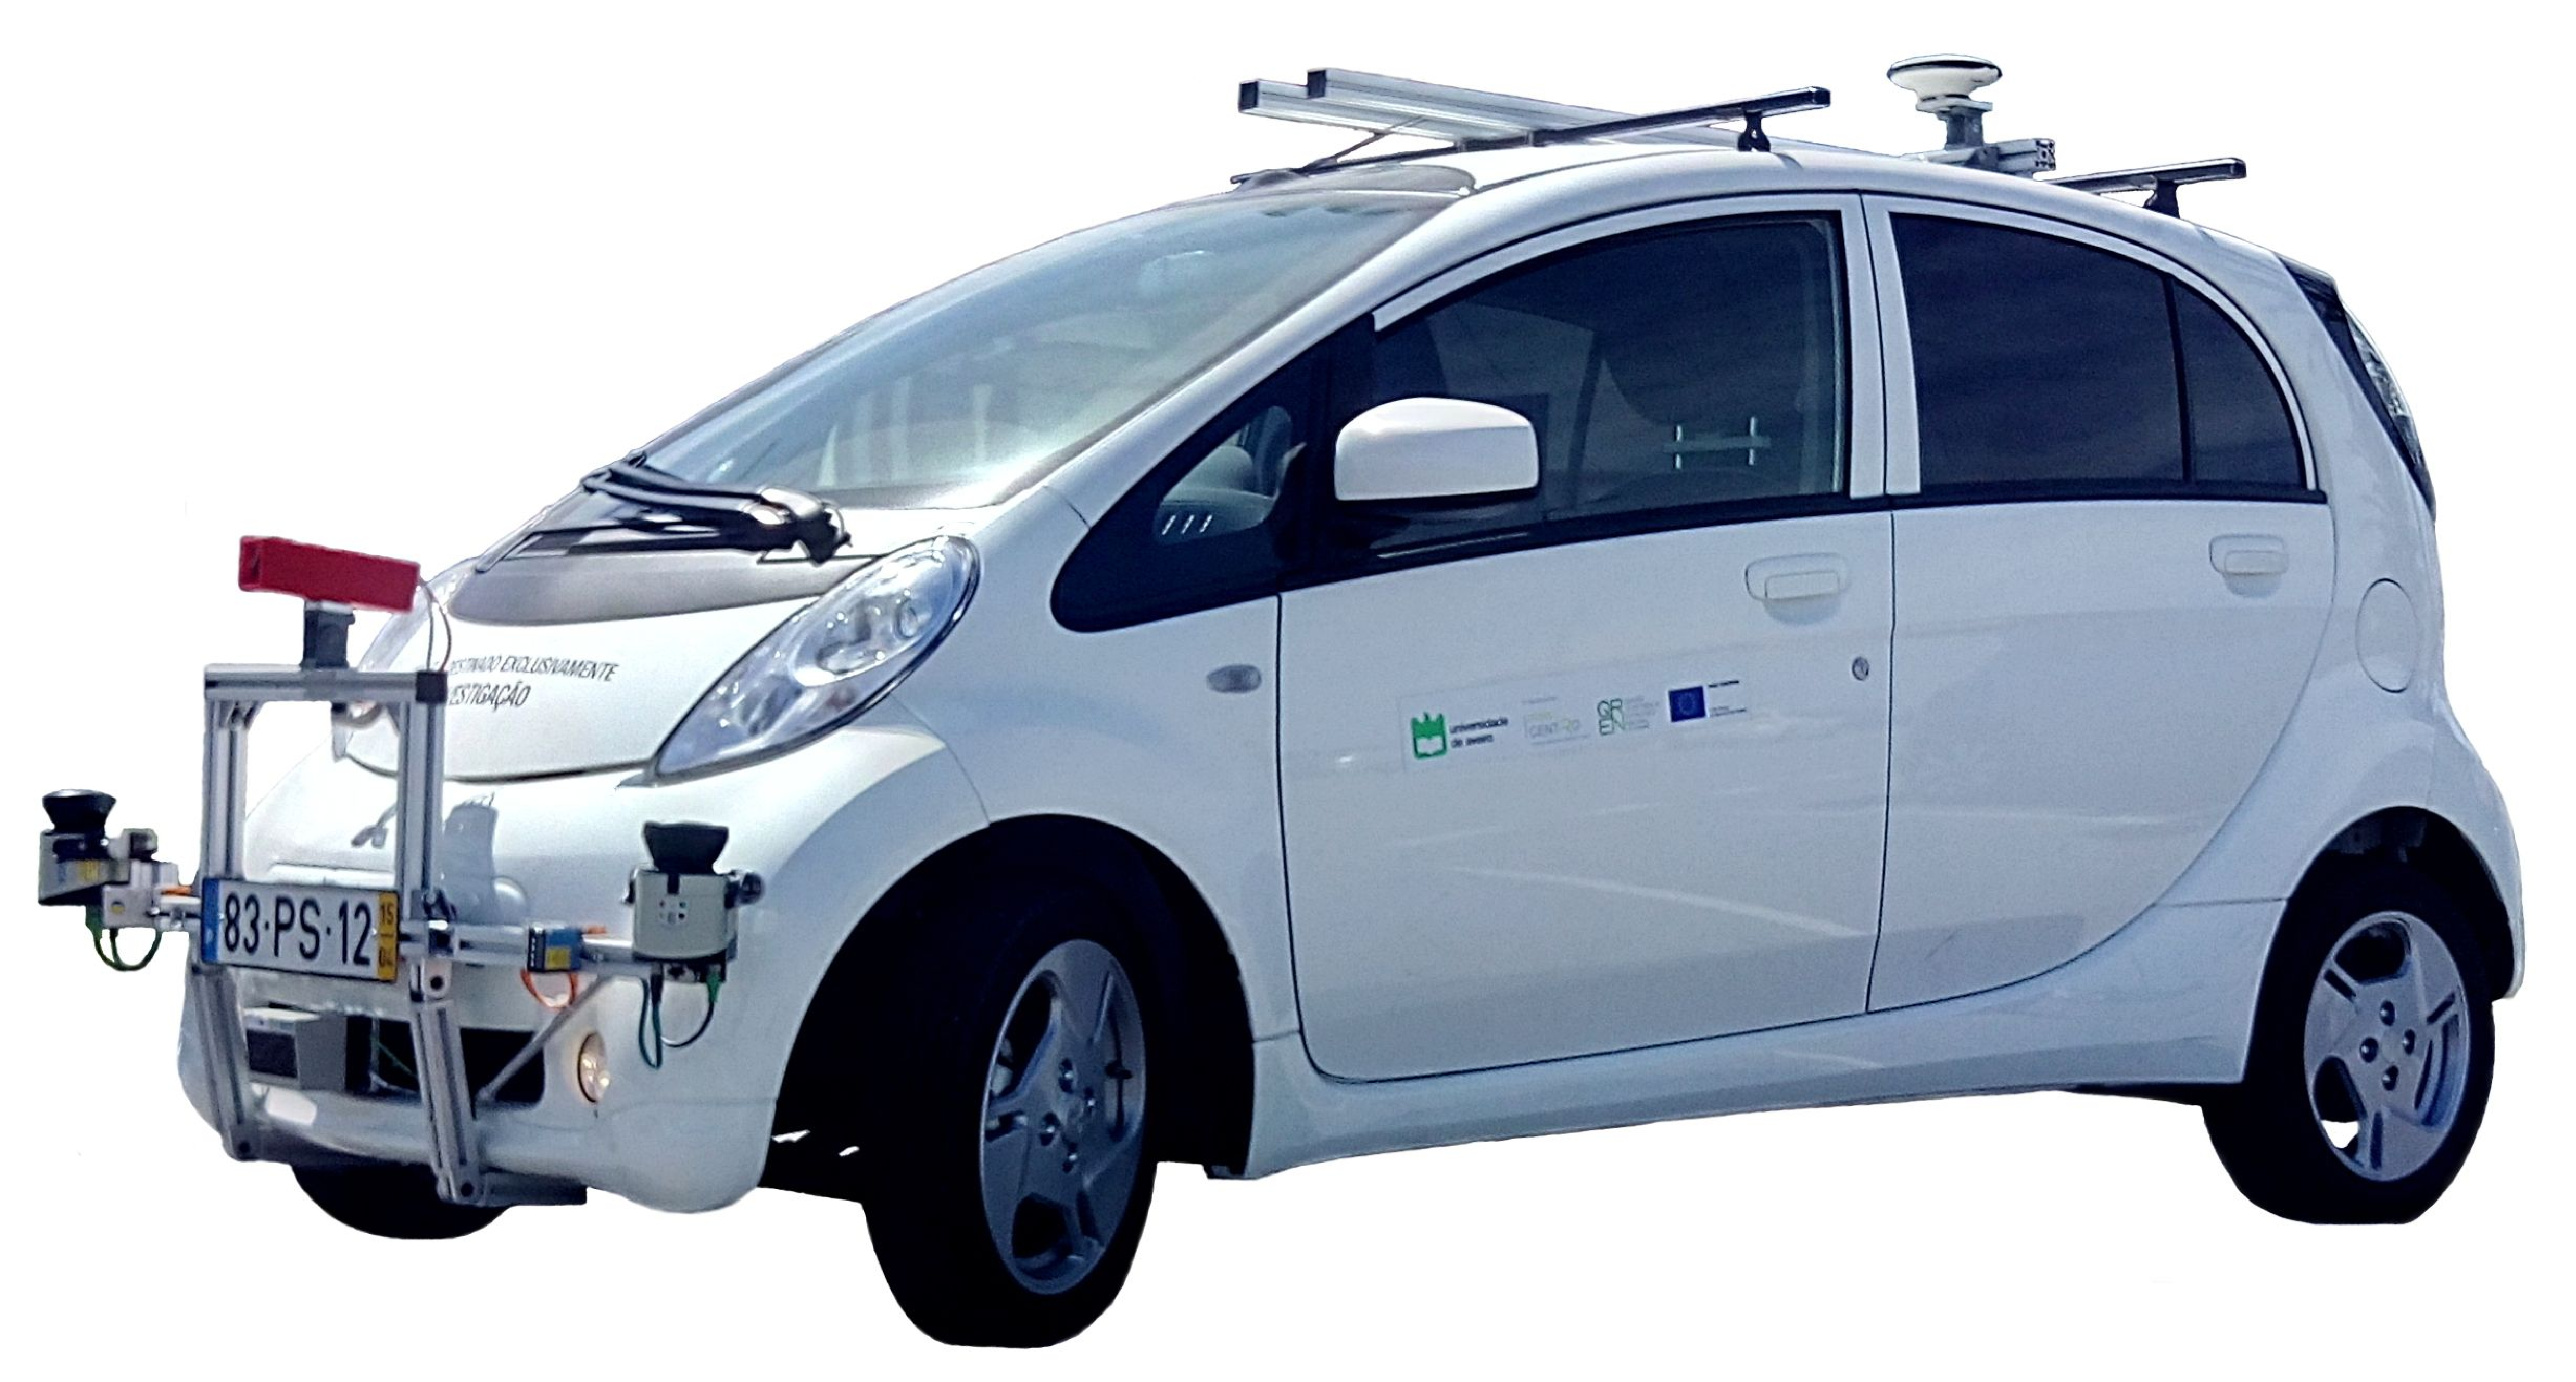
\includegraphics[scale=0.055]{./images/atlascar2.pdf}
	  		\label{fig:atlascar2}
	  	\end{minipage}
	  	\caption{ATLASCAR2 - Mitsubishi iMiEV elettrica del 2015}
	  	\end{figure}

	\end{frame}

	\begin{frame}{Motivazione e Obiettivi della Tesi}
		
	\end{frame}


	\begin{frame}{Model Predictive Control}
		\begin{block}{Normal block}
			Fusce luctus venenatis felis quis semper
		\end{block}

		\begin{alertblock}{Alert block}
			$$ E = (x_1 \vee \neg x_2 \vee \neg x_3) \wedge (x_1 \vee x_2 \vee x_4) $$
		\end{alertblock}

		\begin{exampleblock}{Example block}
			Proin tincidunt, neque at tincidunt mollis
		\end{exampleblock}
	\end{frame}
	
	\section{Moving Obstacle Avoidance System {\itshape \large (sistema di anticollisione con ostacoli in movimento)}} % ovvero un sistema di anticollisione con ostacoli in movimento.
		
	\begin{frame}{Formulazione del Problema} 
	
	\end{frame}
	
	\begin{frame}{Design Adaptive MPC - parte 1} % progettazione dell'algoritmo di anticollisione basato su un controllore MPC adattivo.
		
	\end{frame}
	
	\begin{frame}{Design Adaptive MPC - parte 2} % progettazione dell'algoritmo di anticollisione basato su un controllore MPC adattivo.
		
	\end{frame}
	
	\begin{frame}{Risultati Simulativi}
		
	\end{frame}
	
	\section{Lane Following System \qquad\qquad{\itshape\large(sistema di assistenza al mantenimento della corsia)}}  % ovvero un sistema di assistenza al mantenimento della corsia.
	
	\begin{frame}{Formulazione del Problema}

	\end{frame}
	
	\begin{frame}{Design Adaptive MPC} % progettazione dell'algoritmo di mantenimento della corsia basato su un controllore MPC adattivo.
			
	\end{frame}
		
	\begin{frame}{Risultati Simulativi}
			
	\end{frame}
	\begin{frame}{Conclusioni e Sviluppi Futuri}
		contenuto...
	\end{frame}

\end{document}
